\section{Introduction}

Recommendation systems are a vital component of the modern Web.  They
help readers effectively navigate otherwise unwieldy archives of
information and help websites direct users to items---movies,
articles, songs, products---that they will like.

A recommendation system is built from user behavior data, historical
data about which items each user has consumed, be it clicked, viewed,
rated, or purchased. First, we uncover the behavioral patterns that
characterize various types of users and the kinds of items they tend
to like.  Then, we exploit these discovered patterns to recommend
future items to its users.

In this paper, we develop Poisson factorization (PF) algorithms for
recommendation.  Our algorithms easily scale to massive data and
significantly outperform the existing state of the art.  We show that
Poisson factorization for recommendation is tailored to real-world
properties of user behavior data: the heterogenous interests of users,
the varied types of items, and a realistic distribution of the finite
resources that users have to consume items.

Figure 1 illustrates Poisson factorization on data from Netflix.  The
Netflix data contains the ratings of 480,000 users on 17,000 movies,
organized in a matrix of 8.16B cells (and containing 250M ratings).
From these data, we extract the patterns of users' interests and the
movies that are associated with those interests.  The left panel
ilustrates some of those patterns---the algorithm has uncovered genres
of comedies, classic movies, and 1980s stoner movies.

The middle panel illustrates how we can use these patterns to form
recommendations for an (imaginary) user.  This user enjoys various
types of movies, including war movies (like ``Breaker Morant'') and
romantic dramas (like ``Leaving Las Vegas'').  Of course, she has only
seen a handful of the available movies.  PF first uses the movies she
has seen to infer what kinds of movies she is interested in, and then
uses these inferred interests to suggest movies she has not yet seen.
The list of movies at the bottom of the figure was suggested by our
algorithm. It includes other war dramas (such as ``Apocalypse Now'')
and other romantic movies (such as ``Breakfast at Tiffany's'').

To readers familiar with recommendation systems, this procedure
describes any type of matrix factorization method.  The right panel of
Figure 1 illustrates the quantitative advantages of PF algorithms over
the natural algternatives, based on average per-user precision on
held-out movies.  PF (and its hierarchical variant HPF) performs
significantly better than state-of-the art methods, including
probabilistic matrix factorization (PMF), which is the workhorse
method of most deployed systems.  In our full evaluation, we studied
PF and HPF on many types of large user-behavior data sets: users
watching movies, users reading newspaper articles, users reading
scientific articles, and users listening to music (see \mysec{eval}).
We found significant gains in performance across all the data we
studied, both for data with implicit feedback (a binary data of user
behavior) and data with explicit feedback (a matrix of integer
ratings).

In more detail, Poisson factorization is a probabilistic model of
users and items.  It associates each user with a latent vector of
preferences, each item with a latent vector of attributes, and
constrains both sets of vectors to be sparse and non-negative.  Each
cell of the observed behavior matrix is assumed drawn from a Poisson
distribution---an exponential family distribution over non-negative
integers---whose parameter is a linear combination of the
corresponding user preferences and item attributes.  The main
computational problem is posterior inference: given an observed matrix
of user behavior, we discover the latent attributes that describe the
items and the latent preferences of the users in terms of those
attributes.  For example, the components in Figure 1 (left) illustrate
the top items for specific attribute dimensions and the plot in Figure
1 (middle) illustrates the estimated preference vector for the given
user.  A spike in the preference vector means that the user likes
items with that latent attribute.

There are two main advantages of Poisson factorization, both of which
contribute to its superior empirical performance.  First, it better
captures real consumption data, specifically that users have finite
(and varied) resources with which to view items.  To see this, we can
rewrite the model as a two stage process where a user first decides on
a budget of movies to watch and then spends this budget watching
movies that she is interested in.  If the model accurately captures
the distribution of budgets, then watched items carry more weight than
unwatched items because unwatched items can be partially explained by
a lack of resources.

We conjecture that classical matrix factorization fails on implicit
data because of its poor fit to user budgets, and we will investigate
this hypothesis using posterior predictive checks~\cite{Gelman:1996}.
This issue is why practitioners require complex methods for
downweighting the zeros in the user behavior
matrix~\cite{Hu:2008p9402,Gantner:2012p9364,Dror:2012a,Paquet:2013p9197}.
(We used one such method when comparing to PMF in Figure 1 and in the
full study.)  Poisson factorization does not need to be patched in
this way.

The second advantage of PF algorithms is that they need only iterate
over the viewed items in the observed matrix of user behavior, i.e.,
the non-zero elements.  (This follows from the mathematical form of
the Poisson distribution.)  Thus, Poisson factorization takes
advantage of the natural sparsity of user behavior data and can easily
analyze massive real-world data.  In contrast, classical matrix
factorization, which is based on the Gaussian
distribution~\cite{Salakhutdinov:2008} (i.e., squared loss), iterates
over the entire matrix (especially with implicit data).  It does not
take advantage of sparse data, and this makes computation difficult
for even modestly sized problems.  For example, one cannot fit to the
full Netflix data set (as in Figure 1) without appealing to stochastic
optimization~\cite{Mairal:2010}.  We note that our algorithms are also
amenable to stochastic optimization, which we can use for for data
sets even larger than those we analyzed.

\begin{figure*}[th]
\centering
\caption{The top 5 movies in each of the top 4 components of the user
  $U$ illustrated in Fig~\ref{fig:movielens-illustration}.}
\vspace{0.1cm}
\small
\begin{tabular}{c}
\toprule
\bf{``Drama, Romance''}\\
\midrule
Breakfast at Tiffany's\\
Casablanca\\
The Graduate\\
Shakespeare in Love\\
The African Queen\\
\bottomrule
\end{tabular}
\begin{tabular}{c}
\toprule
\bf{``Drama''}\\
\midrule
Jean de Florette\\
Manon of the Spring\\
Diva\\
The Return of Martin Guerre\\
Blue Velvet\\
\bottomrule
\end{tabular}
\begin{tabular}{c}
\toprule
\bf{``Children's Drama''}\\
\midrule
The Secret Garden\\
The Secret of Roan Inish\\
A Little Princess\\
Fly Away Home\\
Black Beauty\\
\bottomrule
\end{tabular}
\begin{tabular}{c}
\toprule
\bf{``Drama, War''}\\
\midrule
The Bridge on the River Kwai\\
The Right Stuff\\
Patton\\
The Killing Fields\\
Gandhi\\
\bottomrule
\end{tabular}

\end{figure*}

\begin{figure}
\centering
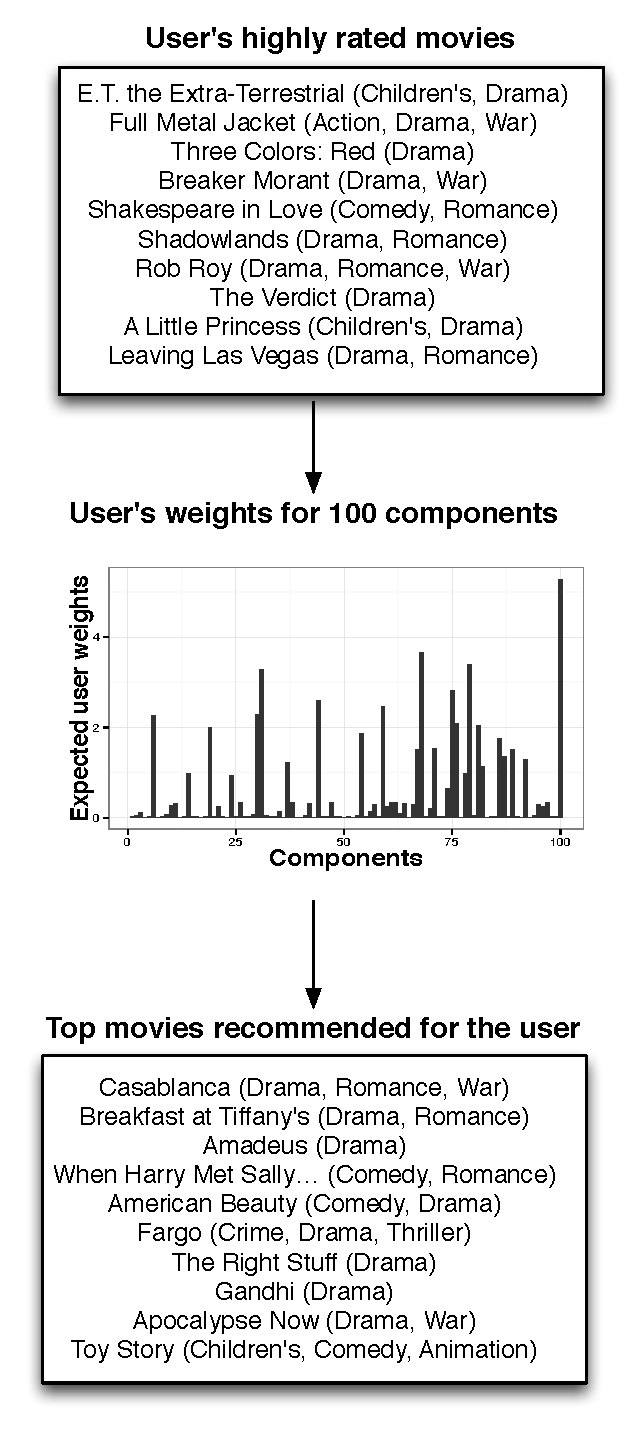
\includegraphics[width=0.8\columnwidth]{figures/movielens-user2.pdf}\\
\caption{An illustration showing a subset of the highly rated movies
  of a selected user $U$ in the MovieLens data set~\cite{Herlocker:1999},
  and a subset of the movies in the top 15 recommended to the user by
  our algorithm. The expected user's $K$-vector of weights $\theta_u$,
  inferred by our algorithm is shown. In our analysis, $K$ was set to
  100.}
\label{fig:movielens-illustration}
\end{figure}


%%
%%\begin{figure}
%%\centering
%%\includegraphics[width=0.8\columnwidth]{figures/movielens-user.pdf}\\
%%\includegraphics[width=0.8\columnwidth]{figures/movielens-item.pdf}\\
%%\caption{The weights of the randomly chosen user $U$ (Top) in the
 %% movielens data set and the weights of her top recommended movie
  %%\emph{Shakespeare in Love} (Bottom) are shown. User $U$ views a
  %%variety of movies, and her weights span a range of factor. User $U$
  %%had 184 views in the data set of movies ranging from Drama, Comedy,
  %%Thriller to Musical. Of these movies, 126 were either 4 or 5
  %%stars. Movies are generally characterized by a sparse set of
  %%factors.}
%%\end{figure}


% Currently, the workhorse method for recommendation systems is matrix
% factorization (MF). MF represents users and items with low
% dimensional vectors and computes the affinity between a user and
% item (that is, whether the user will like it) with the dot product
% of their respective representations.  MF is typically fit with
% squared loss, where the algorithm finds representations that
% minimize the squared difference between the predicted value and the
% observed rating.  (This corresponds to a Gaussian model of the
% data~\cite{Salakhutdinov:2008}.)  MF has been extended in many ways
% to implement modern recommendation
% systems~\cite{Dror:2012,Koren:2008,Rendle:2009,Stern:2009p9238}.

% However, the assumptions behind traditional MF are fundamentally
% flawed when analyzing real-world user behavior data.  In real-world
% data, each user has only rated a small subset of the large population
% of available items. An item a user did \textit{not} rate can arise in
% two ways: either she considered it and chose not to rate it or she did
% not consider it at all.  Each user has a limited budget (of money,
% attention, or time) and therefore most of the unrated items in the
% matrix arise from users not considering (as opposed to actively disliking) them.

% The issue with traditional MF is that it treats all the missing
% cells as observations, as though every user has enough attention to
% consider every available item and decide whether to rate it.  Thus,
% the missing cells are seen as evidence for users not liking the
% items, and this significantly biases the learned representations.
% To address the problem, researchers have patched MF in a variety of
% ways, for example by artificially down-weighting the contribution of
% the unrated items~\cite{Hu:2008p9402}, by sub-sampling from the
% unrated items to give equal weight to the rated
% items~\cite{Gantner:2012p9364,Dror:2012a}, or by explicitly modeling
% the unrated items as missing data~\cite{Paquet:2013p9197}.

% !!! perhaps include these references in the above?

% This issue is particularly critical when analyzing binary data, such
% as product purchases or webpage clicks.  Binary behavior data records
% whether each user consumed an item but does not provide a rating.
% Building recommendation systems from such matrices is known as
% one-class collaborative filtering or recommendation with implicit
% feedback~\cite{Hu:2008p9402,Paquet:2013p9197}.

% !!! include these references in the above

% In this paper, we develop a Bayesian Poisson factorization model as
% an alternative to traditional MF for building recommendation
% systems.  Our model implicitly assumes that each user has a limited
% budget with which to consume items~\cite{Goodhardt:1984}, and thus
% an item that a user has consumed provides a stronger signal about
% her preferences than an item that a user has not consumed.  With
% several kinds of data sets---users rating
% movies~\cite{Herlocker:1999,Koren:2009}, users listening to
% songs~\cite{Bertin-Mahieux:2011}, and users reading scientific
% papers~\cite{Jack:2010}---we demonstrate that Poisson factorization
% leads to better recommendations than both traditional matrix
% factorization and its variants that adjust for sparse data.

% !!! include these points in the above

% Furthermore, Poisson factorization is computationally more efficient
% than traditional MF.  Most algorithms for fitting MF must iterate over
% all user/item pairs, which is expensive for even modestly-sized user
% behavior matrices and cannot take advantage of the sparsity of the
% data~\cite{Hu:2008p9402}.  (To address this issue, practical
% applications of matrix factorization rely on stochastic
% optimization~\cite{Mairal:2010}.)  In this paper, we derive efficient
% variational inference algorithms for Poisson factorization that take
% advantage of the sparsity of the data. Our algorithms need only
% iterate over the non-zero entries of the user behavior matrix.  This
% lets us handle data at a scale that basic (non-stochastic) MF
% algorithms cannot handle.



\begin{figure*}[t!]
  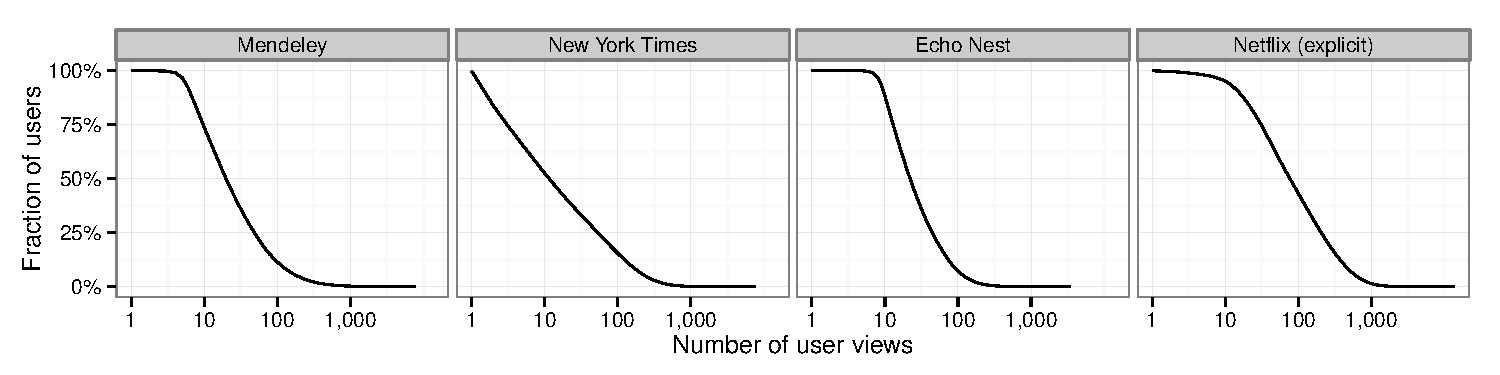
\includegraphics[width=\textwidth]{figures/user_activity_cdf.pdf}
\caption{Empirical complimentary cumulative distributions of user activity on each dataset. Each curve shows the fraction of users who have consumed at least a given number of items. For instance, slightly less than half of all Netflix users have viewed at least 100 movies.}
\label{fig:marginals}
\end{figure*}

%% \begin{figure*}[t!]
%% 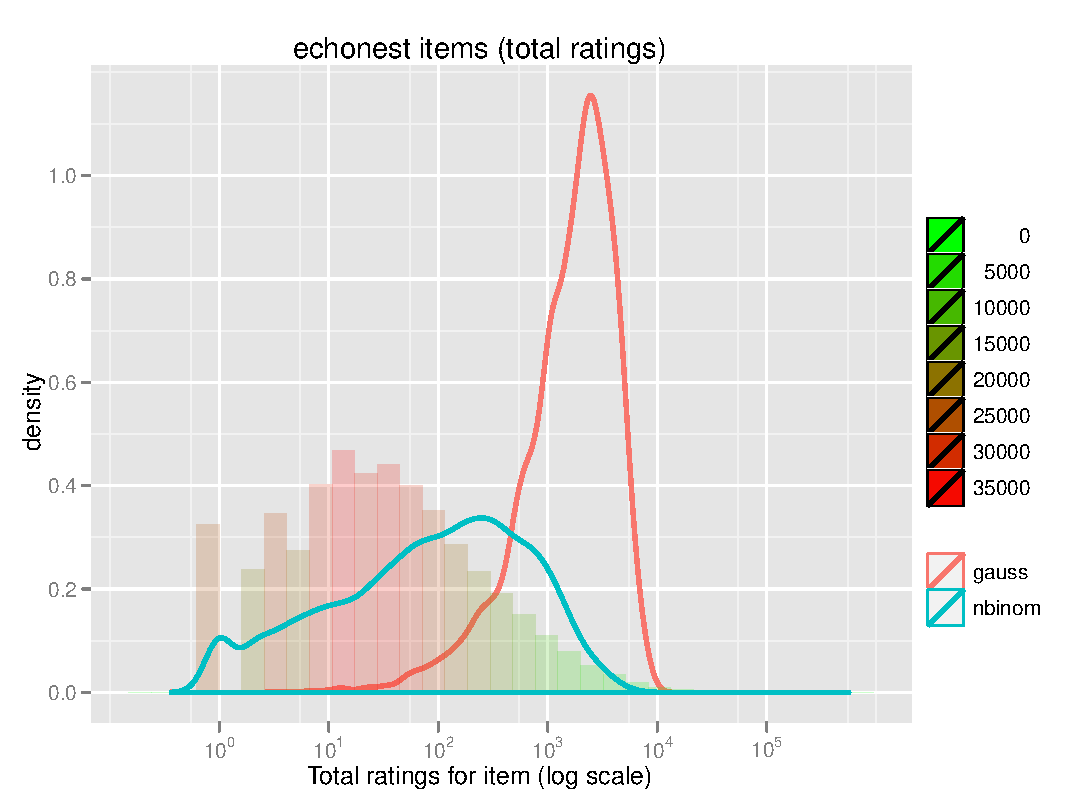
\includegraphics[width=0.33\textwidth]{figures/marginals/echonest.pdf}
%% 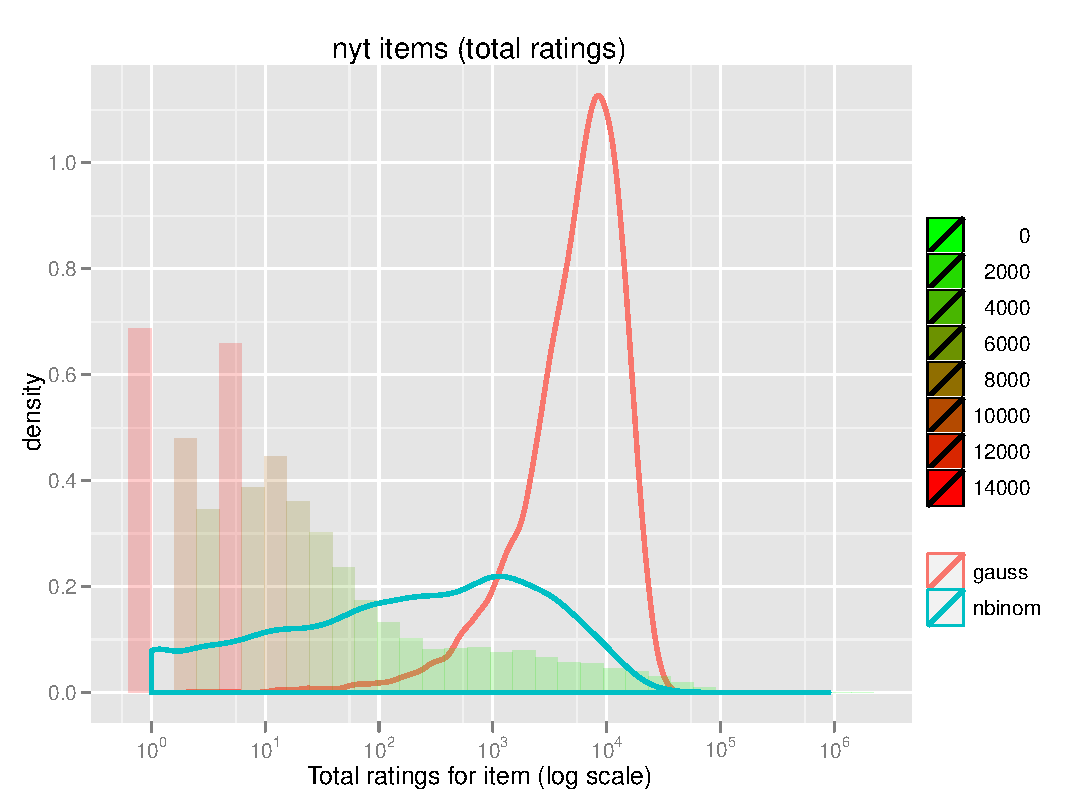
\includegraphics[width=0.33\textwidth]{figures/marginals/nyt.pdf}
%% 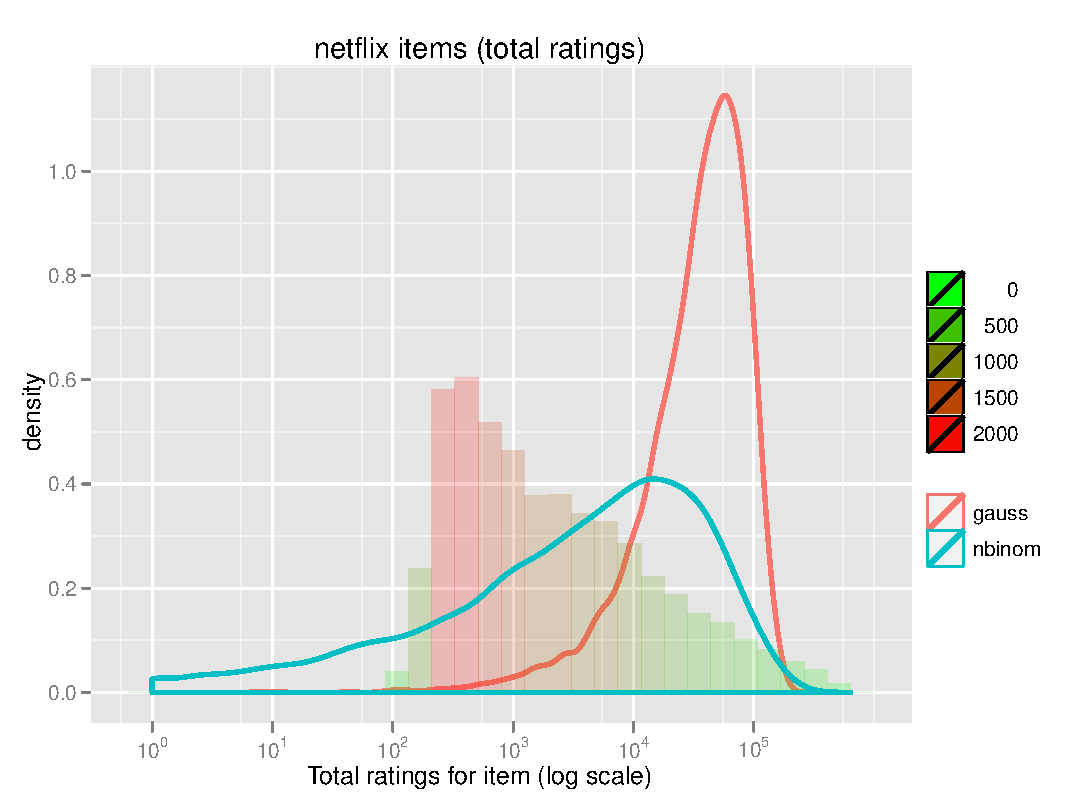
\includegraphics[width=0.33\textwidth]{figures/marginals/netflix.pdf}
%% \caption{Empirical distribution of item popularity on real datasets,
%%   with fitted negative binomial and Gaussian distributions. The
%%   distributions were fit using maximum likelihood estimation. The
%%   negative binomial places significant probability mass on the left
%%   tail, i.e., items with few ratings. The colored bars show that such
%%   items are the most frequent. In contrast, the Gaussian distribution
%%   places negligible mass on the left tail and mainly captures popular
%%   items. The mode of the negative binomial distribution is also closer
%%   to the empirical mode than the Gaussian distribution.}
%% \label{fig:marginals}
%% \end{figure*}

% prem: no longer use stochastic 

%% Further speed-ups using stochastic variational
%% inference~\cite{Hoffman:2013} let us fit Poisson factorization models
%% to massive data.

